% setwd("c:/dev/gbm/inst/doc")
% Sweave("gbm.rnw"); system("texify gbm.tex"); system("c:\\MiKTeX\\texmf\\miktex\\bin\\yap.exe gbm.dvi",wait=FALSE)

\documentclass{article}
\bibliographystyle{plain}
\usepackage[active]{srcltx}
\newcommand{\EV}{\mathrm{E}}
\newcommand{\Var}{\mathrm{Var}}
\newcommand{\aRule}{\begin{center} \rule{5in}{1mm} \end{center}}

\title{Generalized Boosted Models:\\A guide to the gbm package}
\author{Greg Ridgeway}

%\VignetteIndexEntry{Generalized Boosted Models: A guide to the gbm package}
\newcommand{\mathgbf}[1]{{\mbox{\boldmath$#1$\unboldmath}}}

\usepackage{Sweave}
\begin{document}

\maketitle

Boosting takes on various forms with different programs using different loss functions, different base models, and different optimization schemes. The gbm package takes the approach described in \cite{Friedman:2001} and \cite{Friedman:2002}. Some of the terminology differs, mostly due to an effort to cast boosting terms into more standard statistical terminology (e.g. deviance). In addition, the gbm package implements boosting for models commonly used in statistics but not commonly associated with boosting. The Cox proportional hazard model, for example, is an incredibly useful model and the boosting framework applies quite readily with only slight modification \cite{Ridgeway:1999}. Also some algorithms implemented in the gbm package differ from the standard implementation. The AdaBoost algorithm \cite{FreundSchapire:1997} has a particular loss function and a particular optimization algorithm associated with it. The gbm implementation of AdaBoost adopts AdaBoost's exponential loss function (its bound on misclassification rate) but uses Friedman's gradient descent algorithm rather than the original one proposed. So the main purposes of this document is to spell out in detail what the gbm package implements.

\section{Gradient boosting}

This section essentially presents the derivation of boosting described in \cite{Friedman:2001}. The gbm package also adopts the stochastic gradient boosting strategy, a small but important tweak on the basic algorithm, described in \cite{Friedman:2002}.

\subsection{Friedman's gradient boosting machine}
\label{sec:GradientBoostingMachine}

\begin{figure}
\aRule
Initialize $\hat f(\mathbf{x})$ to be a constant, $\hat f(\mathbf{x}) = \arg \min_{\rho} \sum_{i=1}^N \Psi(y_i,\rho)$. \\
For $t$ in $1,\ldots,T$ do
\begin{enumerate}
\item Compute the negative gradient as the working response
    \begin{equation}
    z_i = -\frac{\partial}{\partial f(\mathbf{x}_i)} \Psi(y_i,f(\mathbf{x}_i)) \mbox{\Huge $|$}_{f(\mathbf{x}_i)=\hat f(\mathbf{x}_i)}
    \end{equation}
\item Fit a regression model, $g(\mathbf{x})$, predicting $z_i$ from the covariates $\mathbf{x}_i$.
\item Choose a gradient descent step size as
    \begin{equation}
    \rho = \arg \min_{\rho} \sum_{i=1}^N \Psi(y_i,\hat f(\mathbf{x}_i)+\rho g(\mathbf{x}_i))
    \end{equation}
\item Update the estimate of $f(\mathbf{x})$ as
    \begin{equation}
    \hat f(\mathbf{x}) \leftarrow \hat f(\mathbf{x}) + \rho g(\mathbf{x})
    \end{equation}
\end{enumerate}
\aRule \caption{Friedman's Gradient Boost algorithm}
\label{fig:GradientBoost}
\end{figure}

Friedman (2001) and the companion paper Friedman (2002) extended the work of Friedman, Hastie, and Tibshirani (2000) and laid the ground work for a new generation of boosting algorithms. Using the connection between boosting and optimization, this new work proposes the Gradient Boosting Machine.

In any function estimation problem we wish to find a regression function, $\hat f(\mathbf{x})$, that minimizes the expectation of some loss function, $\Psi(y,f)$, as shown in (\ref{NonparametricRegression1}).
\begin{eqnarray}
\hspace{0.5in}
\hat f(\mathbf{x}) &=& \arg \min_{f(\mathbf{x})} \EV_{y,\mathbf{x}} \Psi(y,f(\mathbf{x})) \nonumber \\
\label{NonparametricRegression1} &=& \arg \min_{f(\mathbf{x})} \EV_x \left[ \EV_{y|\mathbf{x}}
\Psi(y,f(\mathbf{x})) \Big| \mathbf{x} \right]
\end{eqnarray}
We will focus on finding estimates of $f(\mathbf{x})$ such that
\begin{equation}
\label{NonparametricRegression2} \hspace{0.5in} \hat f(\mathbf{x}) = \arg \min_{f(\mathbf{x})}
\EV_{y|\mathbf{x}} \left[ \Psi(y,f(\mathbf{x}))|\mathbf{x} \right]
\end{equation}
Parametric regression models assume that $f(\mathbf{x})$ is a function with a finite
number of parameters, $\beta$, and estimates them by selecting those values
that minimize a loss function (e.g. squared error loss) over a training
sample of $N$ observations on $(y,\mathbf{x})$ pairs as in (\ref{eq:Friedman1}).
\begin{equation}
\label{eq:Friedman1} \hspace{0.5in} \hat\beta = \arg \min_{\beta}
\sum_{i=1}^N \Psi(y_i,f(\mathbf{x}_i;\beta))
\end{equation}
When we wish to estimate $f(\mathbf{x})$ non-parametrically the task becomes more
difficult. Again we can proceed similarly to \cite{FHT:2000} and modify our
current estimate of $f(\mathbf{x})$ by adding a new function $f(\mathbf{x})$ in a greedy
fashion. Letting $f_i = f(\mathbf{x}_i)$, we see that we want to decrease the $N$
dimensional function
\begin{eqnarray}
\label{EQ:Friedman2}
\hspace{0.5in} J(\mathbf{f}) &=& \sum_{i=1}^N \Psi(y_i,f(\mathbf{x}_i)) \nonumber \\
                          &=& \sum_{i=1}^N \Psi(y_i,F_i).
\end{eqnarray}
The negative gradient of $J(\mathbf{f})$ indicates the direction of the
locally greatest decrease in $J(\mathbf{f})$.  Gradient descent would then
have us modify $\mathbf{f}$ as
\begin{equation}
\label{eq:Friedman3} \hspace{0.5in} \hat \mathbf{f} \leftarrow \hat
\mathbf{f} - \rho \nabla J(\mathbf{f})
\end{equation}
where $\rho$ is the size of the step along the direction of greatest descent. Clearly, this step alone is far from our desired goal. First, it only fits $f$ at values of $\mathbf{x}$ for which we have observations.  Second, it does not take into account that observations with similar $\mathbf{x}$ are likely to have similar values of $f(\mathbf{x})$. Both these problems would have disastrous effects on generalization error. However, Friedman suggests selecting a class of functions that use the covariate information to approximate the gradient, usually a regression tree. This line of reasoning produces his Gradient Boosting algorithm shown in Figure~\ref{fig:GradientBoost}. At each iteration the algorithm determines the direction, the gradient, in which it needs to improve the fit to the data and selects a particular model from the allowable class of functions that is in most agreement with the direction. In the case of squared-error loss, $\Psi(y_i,f(\mathbf{x}_i)) = \sum_{i=1}^N (y_i-f(\mathbf{x}_i))^2$, this algorithm corresponds exactly to residual fitting.

There are various ways to extend and improve upon the basic framework suggested in Figure~\ref{fig:GradientBoost}. For example, Friedman (2001) substituted several choices in for $\Psi$ to develop new boosting algorithms for robust regression with least absolute deviation and Huber loss functions. Friedman (2002) showed that a simple subsampling trick can greatly improve predictive performance while simultaneously reduce computation time. Section~\ref{GBMModifications} discusses some of these modifications.

\section{Improving boosting methods using control of the learning rate, sub-sampling, and a decomposition for interpretation}
\label{GBMModifications}

This section explores the variations of the previous algorithms that have the
potential to improve their predictive performance and interpretability. In
particular, by controlling the optimization speed or learning rate,
introducing low-variance regression methods, and applying ideas from robust
regression we can produce non-parametric regression procedures with many
desirable properties. As a by-product some of these modifications lead
directly into implementations for learning from massive datasets. All these
methods take advantage of the general form of boosting
\begin{equation}
\hat f(\mathbf{x}) \leftarrow \hat f(\mathbf{x}) + \EV(z(y,\hat f(\mathbf{x}))|\mathbf{x}).
\end{equation}
So far we have taken advantage of this form only by substituting in our favorite regression procedure for $\EV_w(z|\mathbf{x})$. I will discuss some modifications to estimating $\EV_w(z|\mathbf{x})$ that have the potential to improve our algorithm.

\subsection{Decreasing the learning rate}
As several authors have phrased slightly differently, ``...boosting, whatever flavor, seldom seems to overfit, no matter how many terms are included in the additive expansion''. This is not true as the discussion to \cite{FHT:2000} points out.

In the update step of any boosting algorithm we can introduce a learning rate to dampen the proposed move.
\begin{equation}
\label{eq:shrinkage} \hat f(\mathbf{x}) \leftarrow \hat f(\mathbf{x}) + \lambda \EV(z(y,\hat f(\mathbf{x}))|\mathbf{x}).
\end{equation}
By multiplying the gradient step by $\lambda$ as in equation~\ref{eq:shrinkage} we have control on the rate at which the boosting algorithm descends the error surface (or ascends the likelihood surface). When $\lambda=1$ we return to performing full gradient steps. Friedman (2001) relates the learning rate to regularization through shrinkage.

The optimal number of iterations, $T$, and the learning rate, $\lambda$, depend on each other. In practice I set $\lambda$ to be as small as possible and then select $T$ by cross-validation. Performance is best when $\lambda$ is as small as possible performance with decreasing marginal utility for smaller and smaller $\lambda$. Slower learning rates do not necessarily scale the number of optimal iterations. That is, if when $\lambda=1.0$ and the optimal $T$ is 100 iterations, does {\it not} necessarily imply that when $\lambda=0.1$ the optimal $T$ is 1000 iterations.

\subsection{Variance reduction using subsampling}

Friedman (2002) proposed the stochastic gradient boosting algorithm that simply samples uniformly without
replacement from the dataset before estimating the next gradient step. He found that this additional step greatly improved performance. We estimate the regression $\EV(z(y,\hat f(\mathbf{x}))|\mathbf{x})$ using a random subsample of the dataset.

\subsection{ANOVA decomposition}

Certain function approximation methods are decomposable in terms of a ``functional ANOVA decomposition''.
That is a function is decomposable as
\begin{equation}
\label{ANOVAdecomp} f(\mathbf{x}) = \sum_j f_j(x_j) + \sum_{jk}
f_{jk}(x_j,x_k) + \sum_{jk\ell} f_{jk\ell}(x_j,x_k,x_\ell) + \cdots.
\end{equation}
This applies to boosted trees. Regression stumps (one split decision trees) depend on only one variable and
fall into the first term of \ref{ANOVAdecomp}. Trees with two splits fall into the second term of \ref{ANOVAdecomp} and so on. By restricting the depth of the trees produced on each boosting iteration we can control the order of approximation. Often additive components are sufficient to approximate a multivariate function well, generalized additive models, the na\"{\i}ve Bayes classifier, and boosted stumps for example. When the approximation is restricted to a first order we can also produce plots of $x_j$ versus $f_j(x_j)$ to demonstrate how changes in $x_j$ might affect changes in the response variable.

\subsection{Relative influence}
Friedman (2001) also develops an extension of a variable's ``relative
influence'' for boosted estimates. For tree based methods the approximate
relative influence of a variable $x_j$ is
\begin{equation}
\label{RelInfluence} \hspace{0.5in} \hat J_j^2 =
\hspace{-0.1in}\sum_{\mathrm{splits~on~}x_j}\hspace{-0.2in}I_t^2
\end{equation}
where $I_t^2$ is the empirical improvement by splitting on $x_j$ at that
point. Friedman's extension to boosted models is to average the relative
influence of variable $x_j$ across all the trees generated by the boosting
algorithm.

\begin{figure}
\aRule
Select
\begin{itemize}
\item a loss function (\texttt{distribution})
\item the number of iterations, $T$ (\texttt{n.trees})
\item the depth of each tree, $K$ (\texttt{interaction.depth})
\item the shrinkage (or learning rate) parameter, $\lambda$ (\texttt{shrinkage})
\item the subsampling rate, $p$ (\texttt{bag.fraction})
\end{itemize}
Initialize $\hat f(\mathbf{x})$ to be a constant, $\hat f(\mathbf{x}) = \arg \min_{\rho} \sum_{i=1}^N \Psi(y_i,\rho)$ \\
For $t$ in $1,\ldots,T$ do
\begin{enumerate}
\item Compute the negative gradient as the working response
    \begin{equation}
    z_i = -\frac{\partial}{\partial f(\mathbf{x}_i)} \Psi(y_i,f(\mathbf{x}_i)) \mbox{\Huge $|$}_{f(\mathbf{x}_i)=\hat f(\mathbf{x}_i)}
    \end{equation}
\item Randomly select $p\times N$ cases from the dataset
\item Fit a regression tree with $K$ terminal nodes, $g(\mathbf{x})=\EV(z|\mathbf{x})$. This tree is fit using only those randomly selected observations
\item Compute the optimal terminal node predictions, $\rho_1,\ldots,\rho_K$, as
    \begin{equation}
    \rho_k = \arg \min_{\rho} \sum_{\mathbf{x}_i\in S_k} \Psi(y_i,\hat f(\mathbf{x}_i)+\rho)
    \end{equation}
where $S_k$ is the set of $\mathbf{x}$s that define terminal node $k$.
\item Update $\hat f(\mathbf{x})$ as
    \begin{equation}
    \hat f(\mathbf{x}) \leftarrow \hat f(\mathbf{x}) + \lambda\rho_{k(\mathbf{x})}
    \end{equation}
where $k(\mathbf{x})$ indicates the index of the terminal node into which an observation with features $\mathbf{x}$ would fall. Again this step uses only the randomly selected observations
\end{enumerate}
\aRule \caption{Boosting as implemented in \texttt{gbm()}}
\label{fig:gbm}
\end{figure}

\section{Common user options}

This section discusses the options to gbm that most users will need to change or tune.

\subsection{Loss function}

The first and foremost choice is \texttt{distribution}. This should
be easily dictated by the application. For most classification
problems either \texttt{bernoulli} or \texttt{adaboost} will be
appropriate, the former being recommended. For continuous outcomes
the choices are \texttt{gaussian} (for minimizing squared error),
\texttt{laplace} (for minimizing absolute error), and quantile
regression (for estimating percentiles of the conditional
distribution of the outcome). Censored survival outcomes should
require \texttt{coxph}. Count outcomes may use \texttt{poisson}
although one might also consider \texttt{gaussian} or
\texttt{laplace} depending on the analytical goals.

\subsection{The relationship between shrinkage and number of iterations}
The issues that most new users of gbm struggle with are the choice of \texttt{n.trees} and \texttt{shrinkage}. It is important to know that smaller values of \texttt{shrinkage} (almost) always give improved predictive performance. That is, setting \texttt{shrinkage=0.001} will almost certainly result in a model with better out-of-sample predictive performance than setting \texttt{shrinkage=0.01}. However, there are computational costs, both storage and CPU time, associated with setting \texttt{shrinkage} to be low. The model with \texttt{shrinkage=0.001} will likely require ten times as many iterations as the model with \texttt{shrinkage=0.01}, increasing storage and computation time by a factor of 10. Figure~\ref{fig:shrinkViters} shows the relationship between predictive performance, the number of iterations, and the shrinkage parameter. Note that the increase in the optimal number of iterations between two choices for shrinkage is roughly equal to the ratio of the shrinkage parameters. It is generally the case that for small shrinkage parameters, 0.001 for example, there is a fairly long plateau in which predictive performance is at its best. My rule of thumb is to set \texttt{shrinkage} as small as possible while still being able to fit the model in a reasonable amount of time and storage. I usually aim for 3,000 to 10,000 iterations with shrinkage rates between 0.01 and 0.001.

\begin{figure}[ht]
\begin{center}
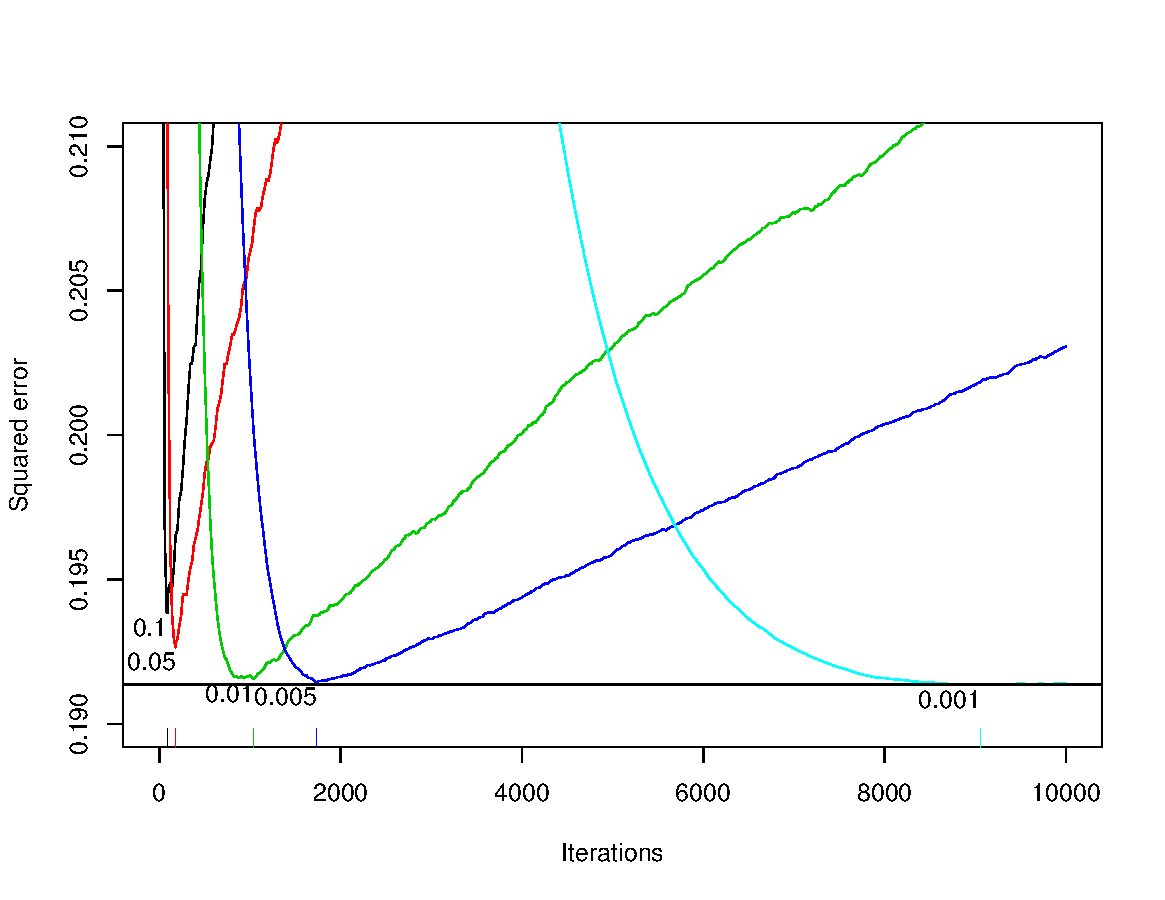
\includegraphics[width=5in]{shrinkage-v-iterations}
\end{center}
\caption{Out-of-sample predictive performance by number of iterations and shrinkage. Smaller values of the shrinkage parameter offer improved predictive performance, but with decreasing marginal improvement.}
\label{fig:shrinkViters}
\end{figure}

\subsection{Estimating the optimal number of iterations}
gbm offers three methods for estimating the optimal number of iterations after the gbm model has been fit, an independent test set (\texttt{test}), out-of-bag estimation (\texttt{OOB}), and $v$-fold cross validation (\texttt{cv}). The function \texttt{gbm.perf} computes the iteration estimate.

Like Friedman's MART software, the independent test set method uses a single holdout test set to select the optimal number of iterations. If \texttt{train.fraction} is set to be less than 1, then only the \textit{first} \texttt{train.fraction}$\times$\texttt{nrow(data)} will be used to fit the model. Note that if the data are sorted in a systematic way (such as cases for which $y=1$ come first), then the data should be shuffled before running gbm. Those observations not used in the model fit can be used to get an unbiased estimate of the optimal number of iterations. The downside of this method is that a considerable number of observations are used to estimate the single regularization parameter (number of iterations) leaving a reduced dataset for estimating the entire multivariate model structure. Use \texttt{gbm.perf(...,method="test")} to obtain an estimate of the optimal number of iterations using the held out test set.

If \texttt{bag.fraction} is set to be greater than 0 (0.5 is recommended), gbm computes an out-of-bag estimate of the improvement in predictive performance. It evaluates the reduction in deviance on those observations not used in selecting the next regression tree. The out-of-bag estimator underestimates the reduction in deviance. As a result, it almost always is too conservative in its selection for the optimal number of iterations. The motivation behind this method was to avoid having to set aside a large independent dataset, which reduces the information available for learning the model structure. Use \texttt{gbm.perf(...,method="OOB")} to obtain the OOB estimate.

Lastly, gbm offers $v$-fold cross validation for estimating the optimal number of iterations. If when fitting the gbm model, \texttt{cv.folds=5} then gbm will do 5-fold cross validation. gbm will fit five gbm models in order to compute the cross validation error estimate and then will fit a sixth and final gbm model with \texttt{n.trees}iterations using all of the data. The returned model object will have a component labeled \texttt{cv.error}. Note that \texttt{gbm.more} will do additional gbm iterations but will not add to the \texttt{cv.error} component. Use \texttt{gbm.perf(...,method="cv")} to obtain the cross validation estimate.

\begin{figure}[ht]
\begin{center}
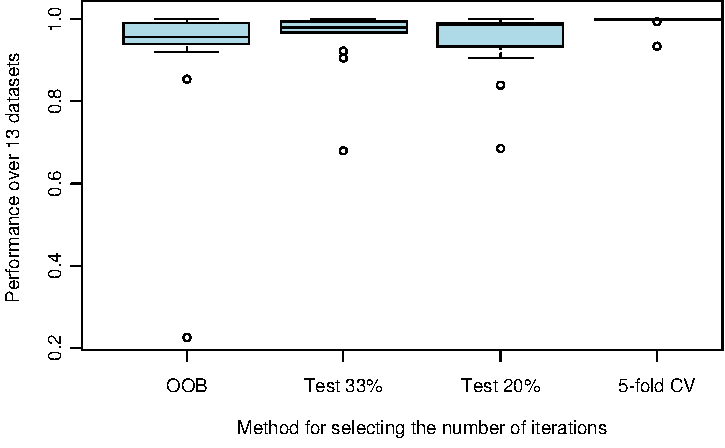
\includegraphics[width=5in]{oobperf2}
\end{center}
\caption{Out-of-sample predictive performance of four methods of selecting the optimal number of iterations. The vertical axis plots performance relative the best. The boxplots indicate relative performance across thirteen real datasets from the UCI repository. See \texttt{demo(OOB-reps)}.}
\label{fig:oobperf}
\end{figure}

Figure~\ref{fig:oobperf} compares the three methods for estimating the optimal number of iterations across 13 datasets. The boxplots show the methods performance relative to the best method on that dataset. For most datasets the method perform similarly, however, 5-fold cross validation is consistently the best of them. OOB, using a 33\% test set, and using a 20\% test set all have datasets for which the perform considerably worse than the best method. My recommendation is to use 5- or 10-fold cross validation if you can afford the computing time. Otherwise you may choose among the other options, knowing that OOB is conservative.

\section{Available distributions}

This section gives some of the mathematical detail for each of the distribution options that gbm offers. The gbm engine written in C++ has access to a C++ class for each of these distributions. Each class contains methods for computing the associated deviance, initial value, the gradient, and the constants to predict in each terminal node.

In the equations shown below, for non-zero offset terms, replace $f(\mathbf{x}_i)$ with $o_i + f(\mathbf{x}_i)$.

\subsection{Gaussian}

\begin{tabular}{ll}
Deviance & $\displaystyle \frac{1}{\sum w_i} \sum w_i(y_i-f(\mathbf{x}_i))^2$ \\
Initial value & $\displaystyle f(\mathbf{x})=\frac{\sum w_i(y_i-o_i)}{\sum w_i}$ \\
Gradient & $z_i=y_i - f(\mathbf{x}_i)$ \\
Terminal node estimates & $\displaystyle \frac{\sum w_i(y_i-f(\mathbf{x}_i))}{\sum w_i}$
\end{tabular}

\subsection{AdaBoost}

\begin{tabular}{ll}
Deviance & $\displaystyle \frac{1}{\sum w_i} \sum w_i\exp(-(2y_i-1)f(\mathbf{x}_i))$ \\
Initial value & $\displaystyle \frac{1}{2}\log\frac{\sum y_iw_ie^{-o_i}}{\sum (1-y_i)w_ie^{o_i}}$ \\
Gradient & $\displaystyle z_i= -(2y_i-1)\exp(-(2y_i-1)f(\mathbf{x}_i))$ \\
Terminal node estimates &
$\displaystyle \frac{\sum (2y_i-1)w_i\exp(-(2y_i-1)f(\mathbf{x}_i))}
      {\sum w_i\exp(-(2y_i-1)f(\mathbf{x}_i))}$
\end{tabular}

\subsection{Bernoulli}

\begin{tabular}{ll}
Deviance & $\displaystyle -2\frac{1}{\sum w_i}
\sum w_i(y_if(\mathbf{x}_i)-\log(1+\exp(f(\mathbf{x}_i))))$ \\
Initial value & $\displaystyle \log\frac{\sum w_iy_i}{\sum w_i(1-y_i)}$ \\
Gradient & $\displaystyle z_i=y_i-\frac{1}{1+\exp(-f(\mathbf{x}_i))}$ \\
Terminal node estimates & $\displaystyle \frac{\sum w_i(y_i-p_i)}{\sum w_ip_i(1-p_i)}$ \\
  & where $\displaystyle p_i = \frac{1}{1+\exp(-f(\mathbf{x}_i))}$ \\
\end{tabular}

Notes:
\begin{itemize}
\item For non-zero offset terms, the computation of the initial value requires Newton-Raphson.
Initialize $f_0=0$ and iterate
$\displaystyle f_0 \leftarrow f_0 + \frac{\sum w_i(y_i-p_i)}{\sum w_ip_i(1-p_i)}$ where
$\displaystyle p_i = \frac{1}{1+\exp(-(o_i+f_0))}$.
\end{itemize}

\subsection{Laplace}

\begin{tabular}{ll}
Deviance & $\frac{1}{\sum w_i} \sum w_i|y_i-f(\mathbf{x}_i)|$ \\
Initial value & $\mbox{median}_w(y)$ \\
Gradient & $z_i=\mbox{sign}(y_i-f(\mathbf{x}_i))$ \\
Terminal node estimates & $\mbox{median}_w(z)$
\end{tabular}

Notes:
\begin{itemize}
\item $\mbox{median}_w(y)$ denotes the weighted median, defined as the solution to the equation $\frac{\sum w_iI(y_i\leq m)}{\sum w_i}=\frac{1}{2}$
\item \texttt{gbm()} currently does not implement the weighted median and issues a warning when the user uses weighted data with \texttt{distribution="laplace"}.
\end{itemize}


\subsection{Quantile regression}

Contributed by Brian Kriegler.

\begin{tabular}{ll}
Deviance & $\frac{1}{\sum w_i}
   \left(\alpha\sum_{y_i>f(\mathbf{x}_i)} w_i(y_i-f(\mathbf{x}_i))\right. +$ \\
         & \hspace{0.5in}$\left.(1-\alpha)\sum_{y_i\leq f(\mathbf{x}_i)} w_i(f(\mathbf{x}_i)-y_i)\right)$ \\
Initial value & $\mathrm{quantile}^{(\alpha)}_w(y)$ \\
Gradient & $z_i=\alpha I(y_i>f(\mathbf{x}_i))-(1-\alpha)I(y_i\leq f(\mathbf{x}_i))$ \\
Terminal node estimates & $\mathrm{quantile}^{(\alpha)}_w(z)$
\end{tabular}

Notes:
\begin{itemize}
\item $\mathrm{quantile}^{(\alpha)}_w(y)$ denotes the weighted quantile, defined
as the solution to the equation
$\frac{\sum w_iI(y_i\leq q)}{\sum w_i}=\alpha$
\item \texttt{gbm()} currently does not implement the weighted median and
issues a warning when the user uses weighted data with
\texttt{distribution=list(name="quantile")}.
\end{itemize}


\subsection{Cox Proportional Hazard}

\begin{tabular}{ll}
Deviance & $-2\sum w_i(\delta_i(f(\mathbf{x}_i)-\log(R_i/w_i)))$\\
Gradient & $\displaystyle z_i=\delta_i - \sum_j \delta_j
            \frac{w_jI(t_i\geq t_j)e^{f(\mathbf{x}_i)}}
                 {\sum_k w_kI(t_k\geq t_j)e^{f(\mathbf{x}_k)}}$ \\
Initial value & 0 \\
Terminal node estimates & Newton-Raphson algorithm
\end{tabular}

\begin{enumerate}
  \item Initialize the terminal node predictions to 0, $\mathgbf{\rho}=0$
  \item Let $\displaystyle
             p_i^{(k)}=\frac{\sum_j I(k(j)=k)I(t_j\geq t_i)e^{f(\mathbf{x}_i)+\rho_k}}
                            {\sum_j I(t_j\geq t_i)e^{f(\mathbf{x}_i)+\rho_k}}$
  \item Let $g_k=\sum w_i\delta_i\left(I(k(i)=k)-p_i^{(k)}\right)$
  \item Let $\mathbf{H}$ be a $k\times k$ matrix with diagonal elements
  \begin{enumerate}
     \item Set diagonal elements $H_{mm}=\sum w_i\delta_i p_i^{(m)}\left(1-p_i^{(m)}\right)$
     \item Set off diagonal elements $H_{mn}=-\sum w_i\delta_i p_i^{(m)}p_i^{(n)}$
  \end{enumerate}
  \item Newton-Raphson update $\mathgbf{\rho} \leftarrow \mathgbf{\rho} - \mathbf{H}^{-1}\mathbf{g}$
  \item Return to step 2 until convergence
\end{enumerate}

Notes:
\begin{itemize}
\item $t_i$ is the survival time and $\delta_i$ is the death indicator.
\item $R_i$ denotes the hazard for the risk set, $R_i=\sum_{j=1}^N w_jI(t_j\geq t_i)e^{f(\mathbf{x}_i)}$
\item $k(i)$ indexes the terminal node of observation $i$
\item For speed, \texttt{gbm()} does only one step of the Newton-Raphson algorithm rather than iterating to convergence. No appreciable loss of accuracy since the next boosting iteration will simply correct for the prior iterations inadequacy.
\item \texttt{gbm()} initially sorts the data by survival time. Doing this reduces the computation of the risk set from $O(n^2)$ to $O(n)$ at the cost of a single up front sort on survival time. After the model is fit, the data are then put back in their original order.
\end{itemize}

\subsection{Poisson}
\begin{tabular}{ll}
Deviance & -2$\frac{1}{\sum w_i} \sum w_i(y_if(\mathbf{x}_i)-\exp(f(\mathbf{x}_i)))$ \\
Initial value & $\displaystyle f(\mathbf{x})= \log\left(\frac{\sum w_iy_i}{\sum w_ie^{o_i}}\right)$ \\
Gradient & $z_i=y_i - \exp(f(\mathbf{x}_i))$ \\
Terminal node estimates & $\displaystyle \log\frac{\sum w_iy_i}{\sum w_i\exp(f(\mathbf{x}_i))}$
\end{tabular}

The Poisson class includes special safeguards so that the most extreme predicted values are $e^{-19}$ and $e^{+19}$. This

\begin{thebibliography}{77}     % start the bibliography

\small                          % put the bibliography in a small font

\bibitem{FreundSchapire:1997}
Y. Freund and R.E. Schapire (1997). ``A decision-theoretic generalization of
on-line learning and an application to boosting,'' \textit{Journal of Computer and System Sciences}, 55(1):119-139.

\bibitem{Friedman:2001}
J.H. Friedman (2001). ``Greedy Function Approximation: A Gradient Boosting
Machine,'' \textit{Annals of Statistics} 29(5):1189-1232.

\bibitem{Friedman:2002}
J.H. Friedman (2002). ``Stochastic Gradient Boosting,'' \textit{Computational Statistics
and Data Analysis} 38(4):367-378.

\bibitem{FHT:2000}
J.H. Friedman, T. Hastie, R. Tibshirani (2000). ``Additive Logistic Regression:
a Statistical View of Boosting,'' \textit{Annals of Statistics} 28(2):337-374.

\bibitem{Ridgeway:1999}
G. Ridgeway (1999). ``The state of boosting,'' \textit{Computing Science and Statistics}
31:172-181.

\end{thebibliography}           % end the bibliography

\end{document}
